%%%%%%%%%%%%%%%%%%%%%%%%%%%%%%%%%%%%%%%%%%%%%%%%%%%%%%%%%%%%%%%%%%%%%%%%%%%%%%%%%
% Maintenance
%%%%%%%%%%%%%%%%%%%%%%%%%%%%%%%%%%%%%%%%%%%%%%%%%%%%%%%%%%%%%%%%%%%%%%%%%%%%%%%%%
\part{Maintenance} \label{Maintenance}

%%%%%%%%%%%%%%%%%%%%%%%%%%%%%%%%%%%%%%%%%%%%%%%%%%%%%%%%%%%%%%%%%%%%%%%%%%%%%%%%
% Cleaning
%%%%%%%%%%%%%%%%%%%%%%%%%%%%%%%%%%%%%%%%%%%%%%%%%%%%%%%%%%%%%%%%%%%%%%%%%%%%%%%%
\chapter{Cleaning} \label{Cleaning}

A dry or slightly damp rag, preferably microfiber, should be sufficient to get
fingerprints, dust and other crud off of the wood finish and \front{} front.

\danger{Do not use alcohol.  Alcohol will ruin the finish.  And to be safe,
don't clean it with any kind of chemical cleaning solution.}

%%%%%%%%%%%%%%%%%%%%%%%%%%%%%%%%%%%%%%%%%%%%%%%%%%%%%%%%%%%%%%%%%%%%%%%%%%%%%%%%
% Disassembly
%%%%%%%%%%%%%%%%%%%%%%%%%%%%%%%%%%%%%%%%%%%%%%%%%%%%%%%%%%%%%%%%%%%%%%%%%%%%%%%%
\chapter{Disassembly} \label{Disassembly}

Disassembly should only be necessary once every several years to change the
\cCC{f}.  The \cMSD{f} should last for quite a while and should not need
replacement for many years.

\par\medskip

Unfortunately, there is no way to add and remove songs from the \cMSD{f} without
disassembly and manually removing the card to do so.  However, it is recommended
that this is kept to a minimum.

%%%%%%%%%%%%%%%%%%%%%%%%%%%%%%%%%%%%%%%%%%%%%%%%%%%%%%%%%%%%%%%%%%%%%%%%%%%%%%%%
% Disassembly - Warnings
%%%%%%%%%%%%%%%%%%%%%%%%%%%%%%%%%%%%%%%%%%%%%%%%%%%%%%%%%%%%%%%%%%%%%%%%%%%%%%%%
\section{Warnings}

Please read and heed these warnings.  The device can be damaged if you do not.

\danger{Be extra careful when removing the screws.  This can't be stressed
enough.  Righty-tighty, lefty-loosey.  If you right-tighty when you should be
lefty-looseying, the screw \textbf{WILL STRIP} the threads in the wood.}

\warning{When removing the screws take note of which screws came out of which
holes.  When initially tapping the holes, threads may have been stripped in one
or more of the holes requiring a deeper hole and a longer screw.}

\danger{Take care when lifting the \cTo{f} off.  The wires attaching the \cTS{f}
and \cCC{f} to the \cMi{f} are attached from the \cTo{f} to the circuit board on
the \cBa{f}.  The wires are long enough to take it off, turn it over and set it
on top of the open enclosure.  But the fit may be tight and it may not simply
come off, and pulling it off too abruptly may result in an upward force
proportional to the frictional force that was making it difficult to pull off in
the first place resulting in the wires getting torn from their connections.}

\danger{Be extra careful when reassembling.  As soon as you feel \textit{any}
pressure when turning a screw - \textbf{STOP}.  If you continue, the threads
in the wood \textbf{WILL BE STRIPPED} and the screw will no longer hold.}

\danger{When reassembling, do \textit{not} rely on the screws pulling the
enclosure together.  Make sure all pieces are tight and flush \textit{before}
tightening the screws.}

\danger{\textbf{DO NOT USE POWER TOOLS}.}

%%%%%%%%%%%%%%%%%%%%%%%%%%%%%%%%%%%%%%%%%%%%%%%%%%%%%%%%%%%%%%%%%%%%%%%%%%%%%%%%
% Disassembly - Tools
%%%%%%%%%%%%%%%%%%%%%%%%%%%%%%%%%%%%%%%%%%%%%%%%%%%%%%%%%%%%%%%%%%%%%%%%%%%%%%%%
\section{Tools}

Only one tool is required - a \mono{3/32"} Hex Driver.  However, it is
recommended that you have handy pencil and paper to keep track of which holes
the screws came out of.

\begin{table}[H]
\ers{1}
\centering
\begin{tabu} { X[1,r,m] | X[6,l,m] }
  \thrule
  \thbi{Quantity} & \thbi{Item} \\ \mrule
  1 & \mono{3/32"} Hex Driver, T-handle or Key \\ \drule{2}
  1 & Pen or pencil \\ \drule{2}
  1 & Piece of paper \\
  \bhrule
\end{tabu}
\end{table}

%%%%%%%%%%%%%%%%%%%%%%%%%%%%%%%%%%%%%%%%%%%%%%%%%%%%%%%%%%%%%%%%%%%%%%%%%%%%%%%%
% Disassembly - Top Removal
%%%%%%%%%%%%%%%%%%%%%%%%%%%%%%%%%%%%%%%%%%%%%%%%%%%%%%%%%%%%%%%%%%%%%%%%%%%%%%%%
\section{Top Removal} \label{Top Removal}

To remove the \cTo{f}, you will need to remove the \num{4} screws that attach
the \cSi{f} to the \cTo{f}.  The order of removal is unimportant.  The \cTo{f}
will then be turned, flipped and placed on top of the enclosure.

\warning{Do the following before proceeding:
\begin{itemize}
  \item Switch the device \sOff{f} using the \hyperref[Power Switch]{\cPo{f}}.
  \item Unplug the \hyperref[Power Adapter]{\cPA{f}}.
\end{itemize}}

%%%%%%%%%%%%%%%%%%%%%%%%%%%%%%%%%%%%%%%%%%%%%%%%%%%%%%%%%%%%%%%%%%%%%%%%%%%%%%%%
% Disassembly - Top Removal - Removing the Screws
%%%%%%%%%%%%%%%%%%%%%%%%%%%%%%%%%%%%%%%%%%%%%%%%%%%%%%%%%%%%%%%%%%%%%%%%%%%%%%%%
\subsection{Removing the Screws} \label{Removing the Screws}

The screws used are technically machine screws which are generally used with
metals, however the wood used for the enclosure is sufficiently dense. Machine
screws are used so that the device can be easily taken apart and put back
together - though care must be taken when doing so.

\par\medskip

Utilizing machine screws as opposed to self-tapping wood screws involves a
different process.  First a hole is drilled, much like a pilot hole for a
self-tapping wood screw, but instead of using a screw driver to drive the screw
in, a tap and tap driver is used to create the threads in the hole.

\par\medskip

Despite the wood being very dense, it is very easy to strip the threads if
overtightned - either when loosening and turning the wrong way or when
tightening.  So go slow, very slow, and as soon as you feel
\textbf{ANY RESISTANCE, STOP TURNING}.

\steps{Removing Screws}{%
\begin{enumerate}
  \item Orient the enclosure so that you are \textit{facing} the screw you
    will be loosening.
  \item Insert the \mono{3/32"} Hex Driver into the head of the screw.
  \item \textit{Slowly} turn \textit{counter-clockwise} until the screw is
    \textit{completely} loosened and pull it out.
  \item Make a note with pencil and paper of the hole the screw came out of and
    place the screw next to or on top of it.
  \item Repeat the above steps for all screws to be removed.
\end{enumerate}}

\begin{figure}[H]
\centering
  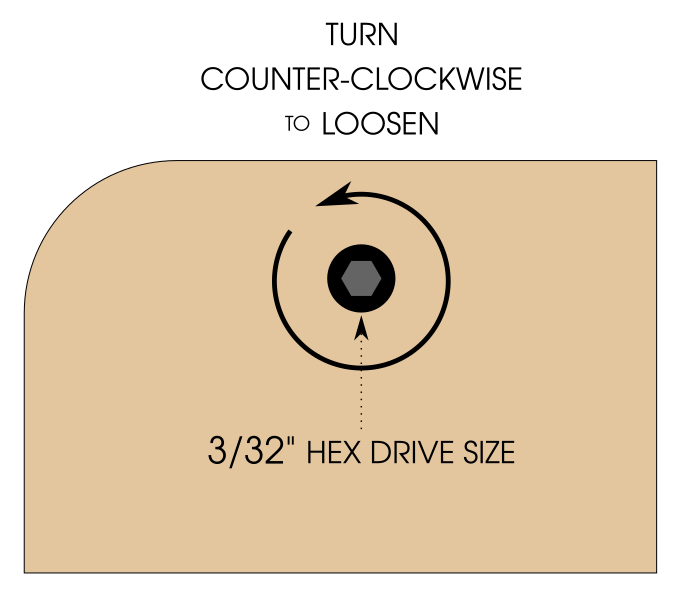
\includegraphics{images/disassembly_loosen.png}
\caption{Disassembly - Loosen Screws}
\end{figure}

\info{If removing the \cMSD{f}, in addition to removing the \num{4} screws
attaching the \cSi{f} to the \cTo{f}, you may need to remove the \num{2} screws
attaching the \cLS{f} to the \cBo{f}.}

%%%%%%%%%%%%%%%%%%%%%%%%%%%%%%%%%%%%%%%%%%%%%%%%%%%%%%%%%%%%%%%%%%%%%%%%%%%%%%%%
% Disassembly - Top Removal - Top Placement
%%%%%%%%%%%%%%%%%%%%%%%%%%%%%%%%%%%%%%%%%%%%%%%%%%%%%%%%%%%%%%%%%%%%%%%%%%%%%%%%
\subsection{Top Placement}

After removing the screws, you will lift the \cTo{f}, turn it over and place
it on top of the enclosure, sitting perpendicular to its attached orientation.

\steps{Top Placement}{%
\begin{enumerate}
  \item \textit{Slowly} pull the \cTo{f} up.  If there is resistance,
    \textit{gently} rock the \cTo{f} from side to side to loosen it until it
    easily detaches.
  \item Lift it \textit{no more} than about \mono{1"} above the enclosure - just
    high enough to be able to turn it perpendicular to the way it is oriented.
  \item Turn the \cTo{f} \textit{counter-clockwise} or to the \textit{left}
    until it is perpendicular to its attached orientation.
  \item Flip it over from \textit{left} to \textit{right}.
  \item \textit{Gently} place it on top of the enclosure.
\end{enumerate}}

\begin{figure}[H]
\centering
  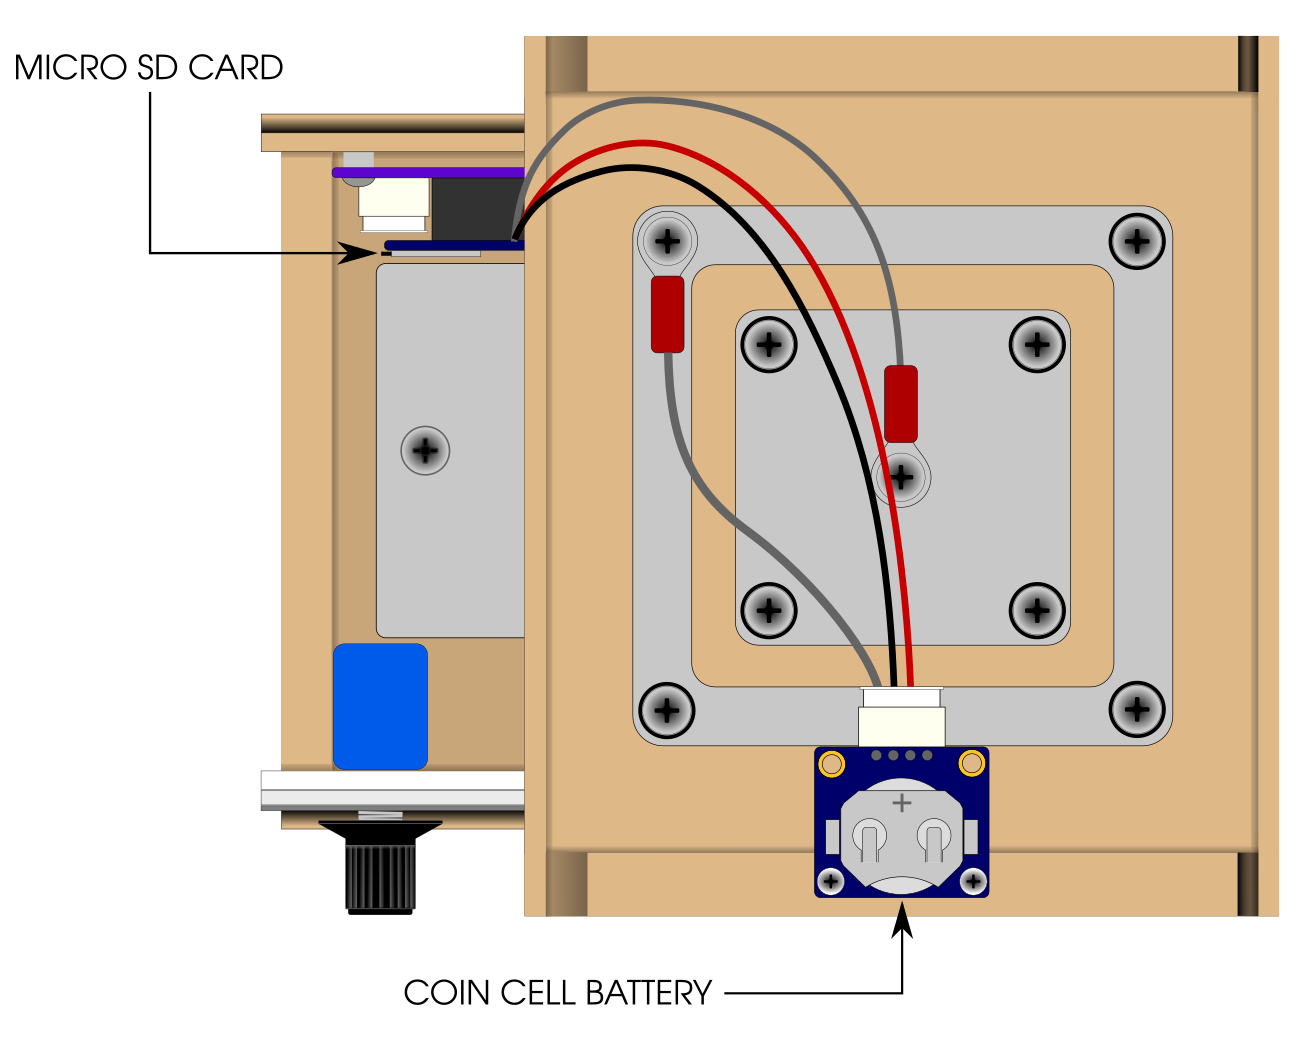
\includegraphics{images/disassembly_placement.png}
\caption{Disassembly - Placement of Top}
\end{figure}

%%%%%%%%%%%%%%%%%%%%%%%%%%%%%%%%%%%%%%%%%%%%%%%%%%%%%%%%%%%%%%%%%%%%%%%%%%%%%%%%
% Disassembly - Reassembly
%%%%%%%%%%%%%%%%%%%%%%%%%%%%%%%%%%%%%%%%%%%%%%%%%%%%%%%%%%%%%%%%%%%%%%%%%%%%%%%%
\section{Reassembly} \label{Reassembly}

Place the \cTo{f} and possibly the \cLS{f}, if it was necessary to remove to
get to the \cMSD{f}, back in place.  Make sure all wires are \textit{within} the
enclosure so that they are not crimped when placing the pieces back together and
that all pieces are tight and flush before putting the screws back in and
tightening.

\par\medskip

Again, go slow, very slow, when tightening the screws and as soon as you feel
\textbf{ANY RESISTANCE, STOP TURNING}.

\steps{Tightening Screws}{%
\begin{enumerate}
  \item Make sure the \cTo{f} and \cSi{f} are tight and flush.
  \item Orient the enclosure so that you are \textit{facing} the screw you
    will be tightening.
  \item Insert the screw into the hole - make sure it is the same screw that
    came out of the hole.
  \item Insert the \mono{3/32"} Hex Driver into the head of the screw.
  \item \textit{Slowly} turn \textit{clockwise}.  As soon as you feel
    \textit{any resistance}, \textbf{STOP} turning.
  \item Repeat the above steps for all removed screws.
\end{enumerate}}

\begin{figure}[H]
\centering
  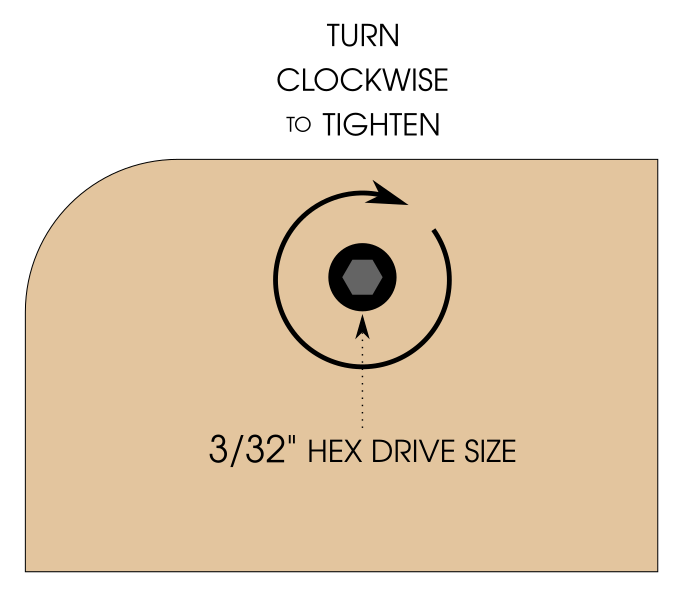
\includegraphics{images/disassembly_tighten.png}
\caption{Reassembly - Tighten Screws}
\end{figure}

%%%%%%%%%%%%%%%%%%%%%%%%%%%%%%%%%%%%%%%%%%%%%%%%%%%%%%%%%%%%%%%%%%%%%%%%%%%%%%%%
% Replacing the Coin Cell Battery
%%%%%%%%%%%%%%%%%%%%%%%%%%%%%%%%%%%%%%%%%%%%%%%%%%%%%%%%%%%%%%%%%%%%%%%%%%%%%%%%
\chapter{Replacing the Coin Cell Battery} \label{Replacing Battery}

Replacing the \hyperref[Coin Cell Battery]{\cCC{f}} shouldn't be necessary for
several years.  It is a \num{CR2032} and is located just underneath the \cTo{f}
on the \textit{left} side.  To access the battery, the \cTo{f} needs to be
removed - refer to the \hyperref[Disassembly]{Disassembly} section for
instructions.

%%%%%%%%%%%%%%%%%%%%%%%%%%%%%%%%%%%%%%%%%%%%%%%%%%%%%%%%%%%%%%%%%%%%%%%%%%%%%%%%
% Replacing the Coin Cell Battery - Parts
%%%%%%%%%%%%%%%%%%%%%%%%%%%%%%%%%%%%%%%%%%%%%%%%%%%%%%%%%%%%%%%%%%%%%%%%%%%%%%%%
\section{Parts}

One \mono{CR2032} coin cell battery is necessary.

\begin{table}[H]
\ers{1}
\centering
\begin{tabu} { X[1,r,m] | X[6,l,m] }
  \thrule
  \thbi{Quantity} & \thbi{Part} \\ \mrule
  1 & \mono{CR2032} (\mono{3\thinspace V}) Coin Cell Battery \\
  \bhrule
\end{tabu}
\end{table}

%%%%%%%%%%%%%%%%%%%%%%%%%%%%%%%%%%%%%%%%%%%%%%%%%%%%%%%%%%%%%%%%%%%%%%%%%%%%%%%%
% Replacing the Coin Cell Battery - Removal
%%%%%%%%%%%%%%%%%%%%%%%%%%%%%%%%%%%%%%%%%%%%%%%%%%%%%%%%%%%%%%%%%%%%%%%%%%%%%%%%
\section{Removal}

To remove the \cCC{f}, simply push it from within the bounds of the \cTo{f}
towards the outside.

\begin{figure}[H]
\centering
  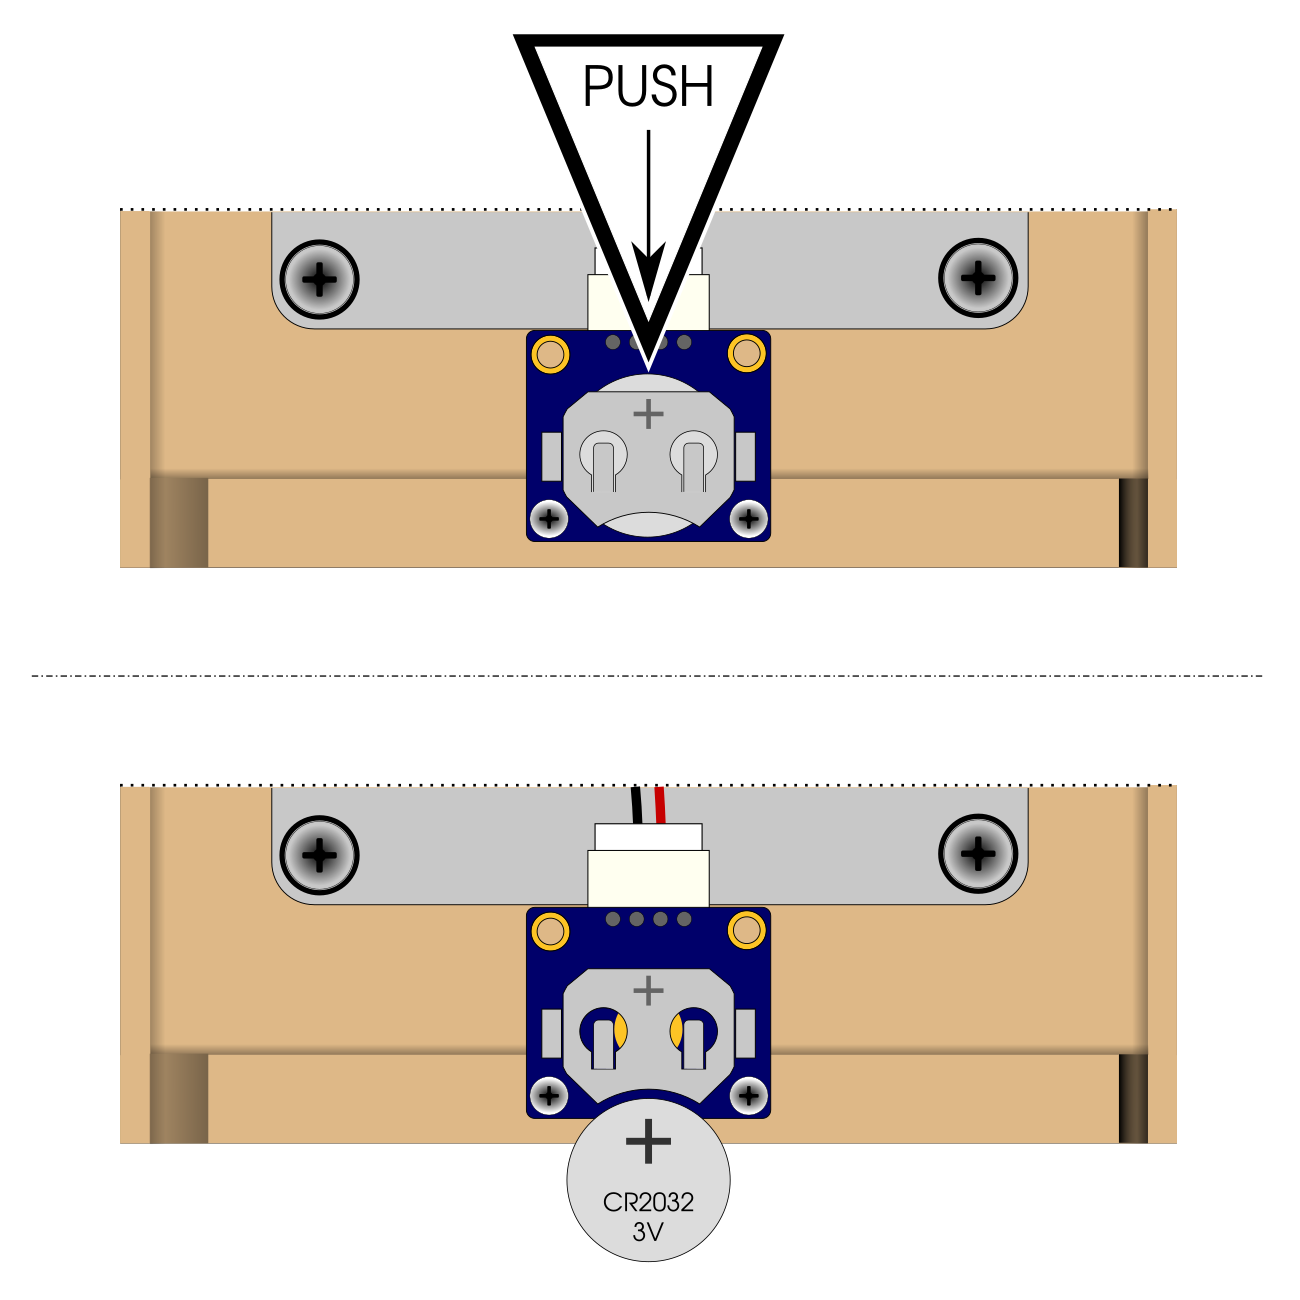
\includegraphics{images/coin_cell_battery.png}
\caption{Removing the Coin Cell Battery}
\end{figure}

%%%%%%%%%%%%%%%%%%%%%%%%%%%%%%%%%%%%%%%%%%%%%%%%%%%%%%%%%%%%%%%%%%%%%%%%%%%%%%%%
% Replacing the Coin Cell Battery - Insertion
%%%%%%%%%%%%%%%%%%%%%%%%%%%%%%%%%%%%%%%%%%%%%%%%%%%%%%%%%%%%%%%%%%%%%%%%%%%%%%%%
\section{Insertion} \label{SD Insertion}

\danger{When inserting the new battery, orientation is critical.  If the
polarity is reversed, damage may occur.}

Before inserting the new battery, make sure the
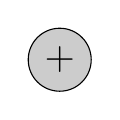
\begin{tikzpicture}[baseline=-4]
  \draw[fill=black!20] (0,0) circle [radius=0.4] node[anchor=center] {\textbf{\Large{$+$}}};
\end{tikzpicture}
or positive side of the battery is \textit{facing up}.  After verifying this,
simply push it in the way it came out.

%%%%%%%%%%%%%%%%%%%%%%%%%%%%%%%%%%%%%%%%%%%%%%%%%%%%%%%%%%%%%%%%%%%%%%%%%%%%%%%%
% Removing the Micro SD Card
%%%%%%%%%%%%%%%%%%%%%%%%%%%%%%%%%%%%%%%%%%%%%%%%%%%%%%%%%%%%%%%%%%%%%%%%%%%%%%%%
\chapter{Removing the Micro SD Card} \label{Removing SD Card}

%Though it's possible and relatively easy to do, the device was not conceived
%to add and remove songs from the \cMSD{f}.

The \cMSD{f} is held in place by a spring clip attached to a part on the circuit
board.  Removal involves pushing the card inward until you hear a
\textit{click}, then releasing.  The card will be partially pushed out by the
spring clip.  You can then pull the card out the rest of the way.  To put the
card back in, push until you hear a \textit{click} and it will catch into place.
Verify that it is in place by gently pulling on it - it should \textit{not} pull
out.

\par\medskip

Before the \cMSD{f} can be removed, the enclosure needs to be partially
disassembled - refer to \hyperref[Disassembly]{Disassembly} for instructions.

\info{You may need to detach the \cLS{f} to get to the card.  If so remove the
\num{2} screws that attach the \cLS{f} to the \cBo{f} in addition to the \num{4}
that attach the \cSi{f} to the \cTo{f} -
see \hyperref[Removing the Screws]{Removing the screws} in the
\hyperref[Top Removal]{Top Removal} section.}

\begin{figure}[H]
\centering
  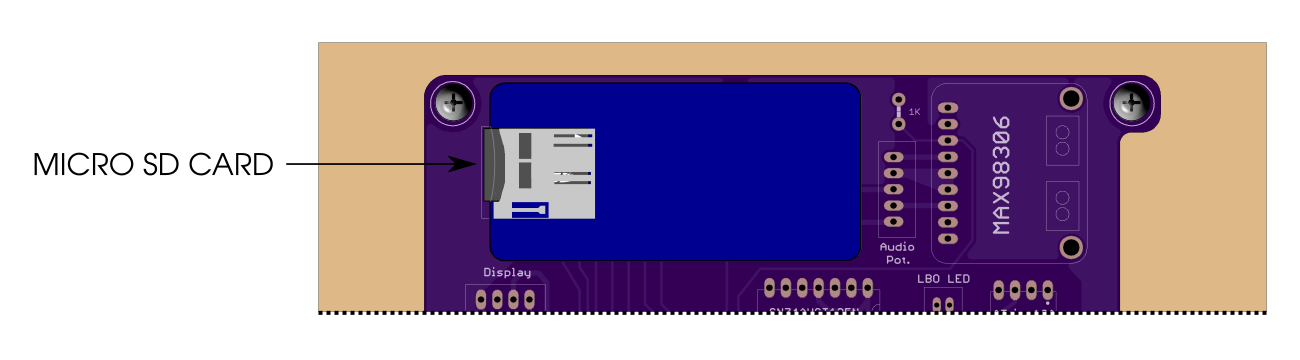
\includegraphics{images/micro_sd_card.png}
\caption{Micro SD Card - Location}
\end{figure}

%%%%%%%%%%%%%%%%%%%%%%%%%%%%%%%%%%%%%%%%%%%%%%%%%%%%%%%%%%%%%%%%%%%%%%%%%%%%%%%%
% Removing the Micro SD Card - Removal
%%%%%%%%%%%%%%%%%%%%%%%%%%%%%%%%%%%%%%%%%%%%%%%%%%%%%%%%%%%%%%%%%%%%%%%%%%%%%%%%
\section{Removal} \label{SD Removal}

To remove the card:

\begin{enumerate}
  \item Push the \cMSD{f} inward until you hear a \textit{click}.
    \begin{figure}[H]
    \centering
      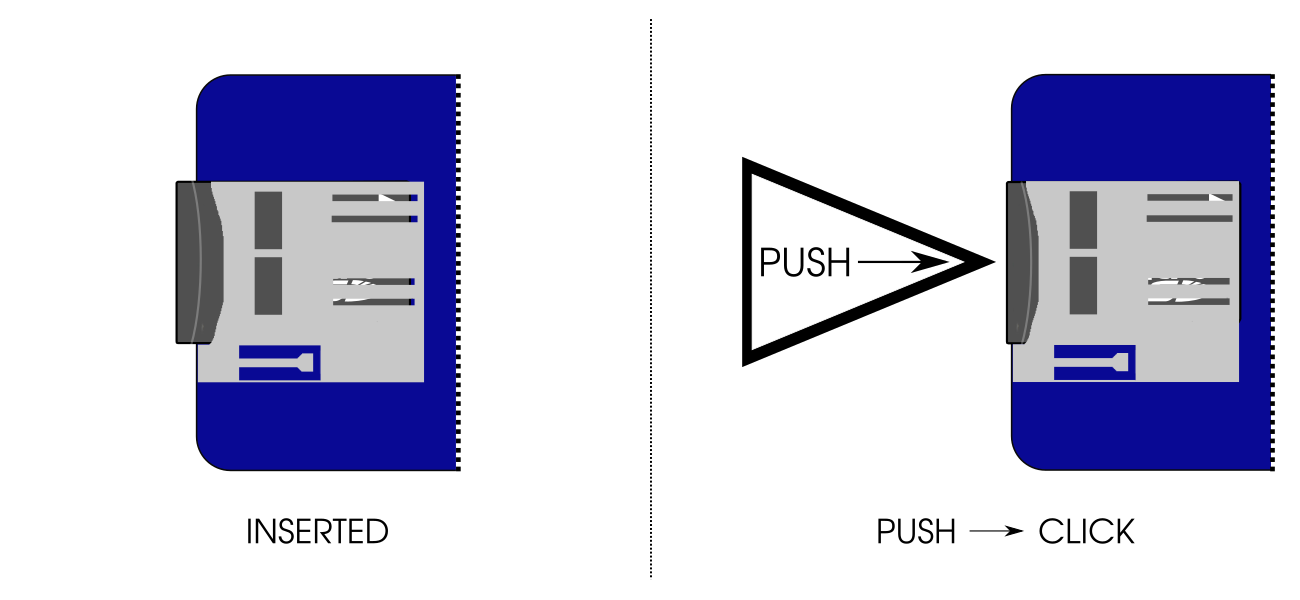
\includegraphics{images/micro_sd_card_removal_01.png}
    \caption{Micro SD Card - Removal (Step 1)}
    \end{figure}
  \item Release and the card will be partially pushed out.
    \begin{figure}[H]
    \centering
      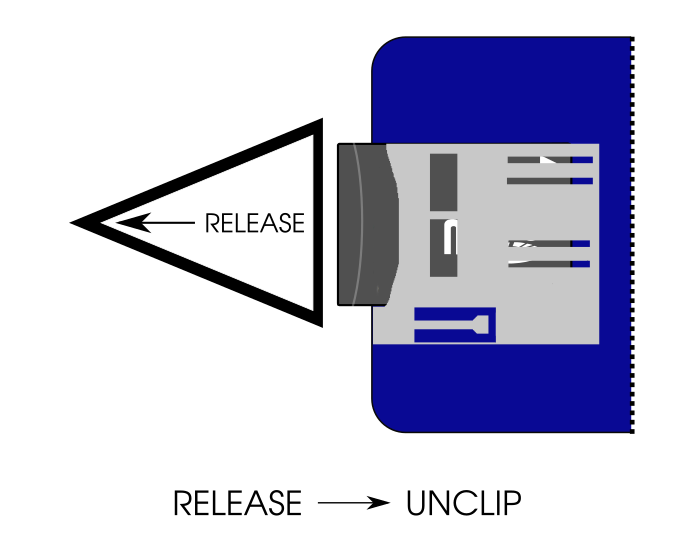
\includegraphics{images/micro_sd_card_removal_02.png}
    \caption{Micro SD Card - Removal (Step 2)}
    \end{figure}
  \item Pull the card out the rest of the way.
    \begin{figure}[H]
    \centering
      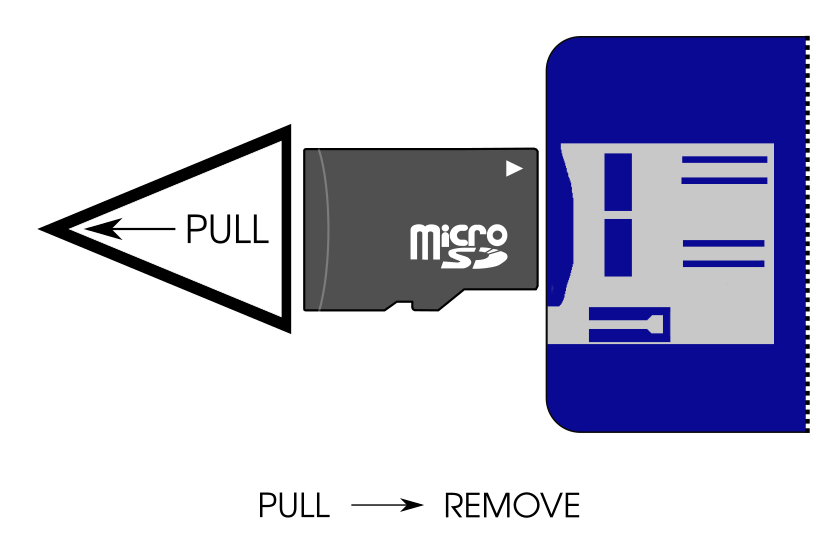
\includegraphics{images/micro_sd_card_removal_03.png}
    \caption{Micro SD Card - Removal (Step 3)}
    \end{figure}
\end{enumerate}

%%%%%%%%%%%%%%%%%%%%%%%%%%%%%%%%%%%%%%%%%%%%%%%%%%%%%%%%%%%%%%%%%%%%%%%%%%%%%%%%
% Removing the Micro SD Card - Insertion
%%%%%%%%%%%%%%%%%%%%%%%%%%%%%%%%%%%%%%%%%%%%%%%%%%%%%%%%%%%%%%%%%%%%%%%%%%%%%%%%
\section{Insertion}

To insert the card:

\begin{enumerate}
  \item Push the \cMSD{f} inward until you hear a \textit{click}.
    \begin{figure}[H]
    \centering
      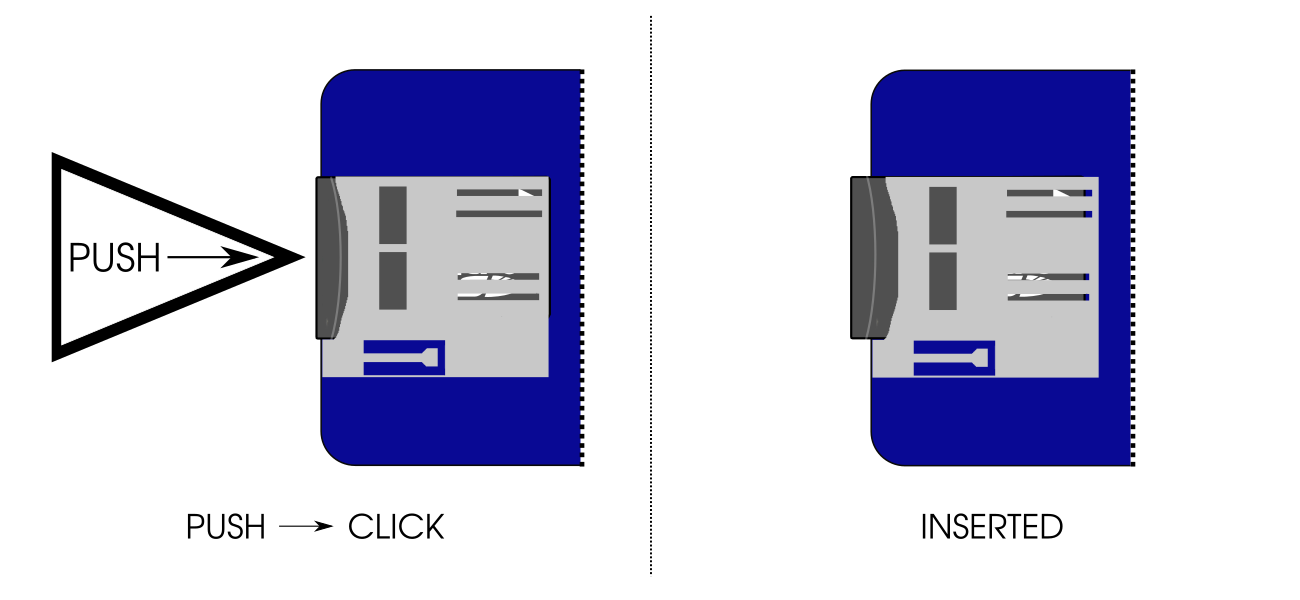
\includegraphics{images/micro_sd_card_insertion.png}
    \caption{Micro SD Card - Insertion}
    \end{figure}
\end{enumerate}

%%%%%%%%%%%%%%%%%%%%%%%%%%%%%%%%%%%%%%%%%%%%%%%%%%%%%%%%%%%%%%%%%%%%%%%%%%%%%%%%
% Removing the Micro SD Card - Adding / Removing Songs
%%%%%%%%%%%%%%%%%%%%%%%%%%%%%%%%%%%%%%%%%%%%%%%%%%%%%%%%%%%%%%%%%%%%%%%%%%%%%%%%
\section{Adding / Removing Songs} \label{Add Songs}

Disassembly is primarily meant for maintenance and changing the \cCC{f}
and should \textit{not} be done often.  Unfortunately the only way to
add / remove songs from the \cMSD{f} is to partially disassemble the enclosure
- see \hyperref[Disassembly]{Disassembly} for instructions.

\par\medskip

The \cMSD{f} can have any number of songs on it, however, the \textit{maximum}
number of songs that the device will be able to play is \num{4096}.

\par\medskip

There are a number of ways to add files to the \cMSD{f}.  It will be assumed
that a desktop or laptop computer with a windowed environment is being used
such as a Mac or Windows.

%%%%%%%%%%%%%%%%%%%%%%%%%%%%%%%%%%%%%%%%%%%%%%%%%%%%%%%%%%%%%%%%%%%%%%%%%%%%%%%%
% Removing the Micro SD Card - Adding / Removing Songs - Preparation
%%%%%%%%%%%%%%%%%%%%%%%%%%%%%%%%%%%%%%%%%%%%%%%%%%%%%%%%%%%%%%%%%%%%%%%%%%%%%%%%
\subsection{Preparation}

Preparation involves partially disassembling the enclosure, removing the
\cMSD{f} from the holder on the circuit board and attaching the card to a
computer.

\steps{Preparation}{%
\begin{enumerate}
  \item Partially disassemble the enclosure - refer to
    \hyperref[Disassembly]{Disassembly} for instructions.
  \item Remove the \cMSD{f} - refer to \hyperref[SD Removal]{Removal} for
    instructions.
  \item Insert the card into the computer.  There are a couple of ways this
    may be accomplished.
    \begin{itemize}
      \item If your computer has a built-in \cMSD{f} reader, you should be
        able to use that.
      \item Use a USB card reader.\footnote{ One that I have used without issue
        is \mono{Transcend RDF5}.}  After inserting the card into the reader,
        insert the reader into a USB port on the computer.
    \end{itemize}
  \item The card should be recognized as a disk volume on the computer.  The
    card that comes pre-installed is named \mono{MUSIC}.  Open a window that
    shows the contents of the disk.
\end{enumerate}}

%%%%%%%%%%%%%%%%%%%%%%%%%%%%%%%%%%%%%%%%%%%%%%%%%%%%%%%%%%%%%%%%%%%%%%%%%%%%%%%%
% Removing the Micro SD Card - Adding / Removing Songs - Adding Files
%%%%%%%%%%%%%%%%%%%%%%%%%%%%%%%%%%%%%%%%%%%%%%%%%%%%%%%%%%%%%%%%%%%%%%%%%%%%%%%%
\subsection{Adding Songs} \label{Adding Songs}

Adding songs involves copying \mono{MP3} or \mono{M4A} music files that are on
a computer to the \cMSD{f}.

\warning{The files \textit{must} be \mono{MPEG-2 Audio Layer III} (\mono{MP3})
or \mono{MPEG-4 Audio}\footnote{ Used primarily by iTunes.} (\mono{M4A}) files
and they \textit{must} have an \mono{.mp3} or \mono{.m4a} file extension.
Files that are \textit{not} \mono{MP3} or \mono{M4A} and that do \textit{not}
have either of the two file extensions in the file name will \textit{not} work.}

\steps{Adding Songs}{%
\begin{enumerate}
  \item Open another window that has the songs you want to add.
  \item Drag and drop the \mono{MP3} and/or \mono{M4A} files you want to add
    onto the \cMSD{f} volume.
    \par\medskip
    Note that the disk has no concept of sorting and the order in which the
    songs are "sorted" on the disk is the order in which they are added to
    the disk.  If you want the songs to be played in a specific order,
    add them \textit{one at a time} to the \cMSD{f}.
\end{enumerate}}

%%%%%%%%%%%%%%%%%%%%%%%%%%%%%%%%%%%%%%%%%%%%%%%%%%%%%%%%%%%%%%%%%%%%%%%%%%%%%%%%
% Removing the Micro SD Card - Adding / Removing Songs - Removing Files
%%%%%%%%%%%%%%%%%%%%%%%%%%%%%%%%%%%%%%%%%%%%%%%%%%%%%%%%%%%%%%%%%%%%%%%%%%%%%%%%
\subsection{Removing Songs}

Removing songs simply involves deleting the files from the \cMSD{f}.

\steps{Removing Songs}{%
\begin{enumerate}
  \item Delete or "Move to Trash" the files you want removed from the
    \cMSD{f} volume.
\end{enumerate}}

%%%%%%%%%%%%%%%%%%%%%%%%%%%%%%%%%%%%%%%%%%%%%%%%%%%%%%%%%%%%%%%%%%%%%%%%%%%%%%%%
% Removing the Micro SD Card - Adding / Removing Songs - Finishing
%%%%%%%%%%%%%%%%%%%%%%%%%%%%%%%%%%%%%%%%%%%%%%%%%%%%%%%%%%%%%%%%%%%%%%%%%%%%%%%%
\subsection{Finishing}

Finishing involves ejecting then physically removing the \cMSD{f} from the
computer, putting it back in the holder on the circuit board and closing up the
enclosure.

\steps{Finishing}{%
\begin{enumerate}
  \item Safely remove or eject the \cMSD{f}. This is \textit{not} physical
    removal but tells the computer to finish any possible pending
    operations, such as writes to the disk, \textit{before} physical removal.
  \item Physically remove the \cMSD{f} from the computer.
  \item Reinsert the \cMSD{f} back into the holder on the circuit board -
    refer to \hyperref[SD Insertion]{Insertion} for instructions.
  \item Reassemble the enclosure - refer to \hyperref[Reassembly]{Reassembly}
    for instructions.
\end{enumerate}}

%%%%%%%%%%%%%%%%%%%%%%%%%%%%%%%%%%%%%%%%%%%%%%%%%%%%%%%%%%%%%%%%%%%%%%%%%%%%%%%%
% Removing the Micro SD Card - Replace SD Card
%%%%%%%%%%%%%%%%%%%%%%%%%%%%%%%%%%%%%%%%%%%%%%%%%%%%%%%%%%%%%%%%%%%%%%%%%%%%%%%%
\section{Replacement} \label{Replace SD Card}

The \cMSD{f} may eventually fail and need to be replaced.  This section will
only focus on formatting the new card.  See the
\hyperref[Disassembly]{Disassembly} section and the preceding sections for
removing the card from the enclosure and adding songs.

\par\medskip

The new card must meet these requirements.

\begin{itemize}
  \item The card \textit{must} have at least a \num{90} \mono{MB/sec} read
    speed, \textit{and}
  \item The card \textit{must} be formatted with the \mono{FAT32} filesystem
    using \num{512} bytes per sector.
\end{itemize}

\warning{If the read speed of the card is less than \num{90} \mono{MB/sec}, the
audio may stutter and not play correctly.}

\danger{If the card is not formatted with the \mono{FAT32} filesystem using
\num{512} bytes per sector, the device will \textit{not} be able to read the
card.}

%%%%%%%%%%%%%%%%%%%%%%%%%%%%%%%%%%%%%%%%%%%%%%%%%%%%%%%%%%%%%%%%%%%%%%%%%%%%%%%%
% Removing the Micro SD Card - Replace SD Card - Parts
%%%%%%%%%%%%%%%%%%%%%%%%%%%%%%%%%%%%%%%%%%%%%%%%%%%%%%%%%%%%%%%%%%%%%%%%%%%%%%%%
\subsection{Parts}

One Micro SD Card with at least a \num{90} \mono{MB/sec} read speed specification
is needed.

\begin{table}[H]
\ers{1}
\centering
\begin{tabu} { X[1,r,m] | X[6,l,m] }
  \thrule
  \thbi{Quantity} & \thbi{Part} \\ \mrule
  1 & Micro SD Card w/ \num{90} \mono{MB/sec} or more Read Speed \\
  \bhrule
\end{tabu}
\end{table}

A Micro SD Card is distinguished from a normal SD card and the Mini SD Card in
that it is the smallest of the three.

\begin{figure}[H]
\centering
  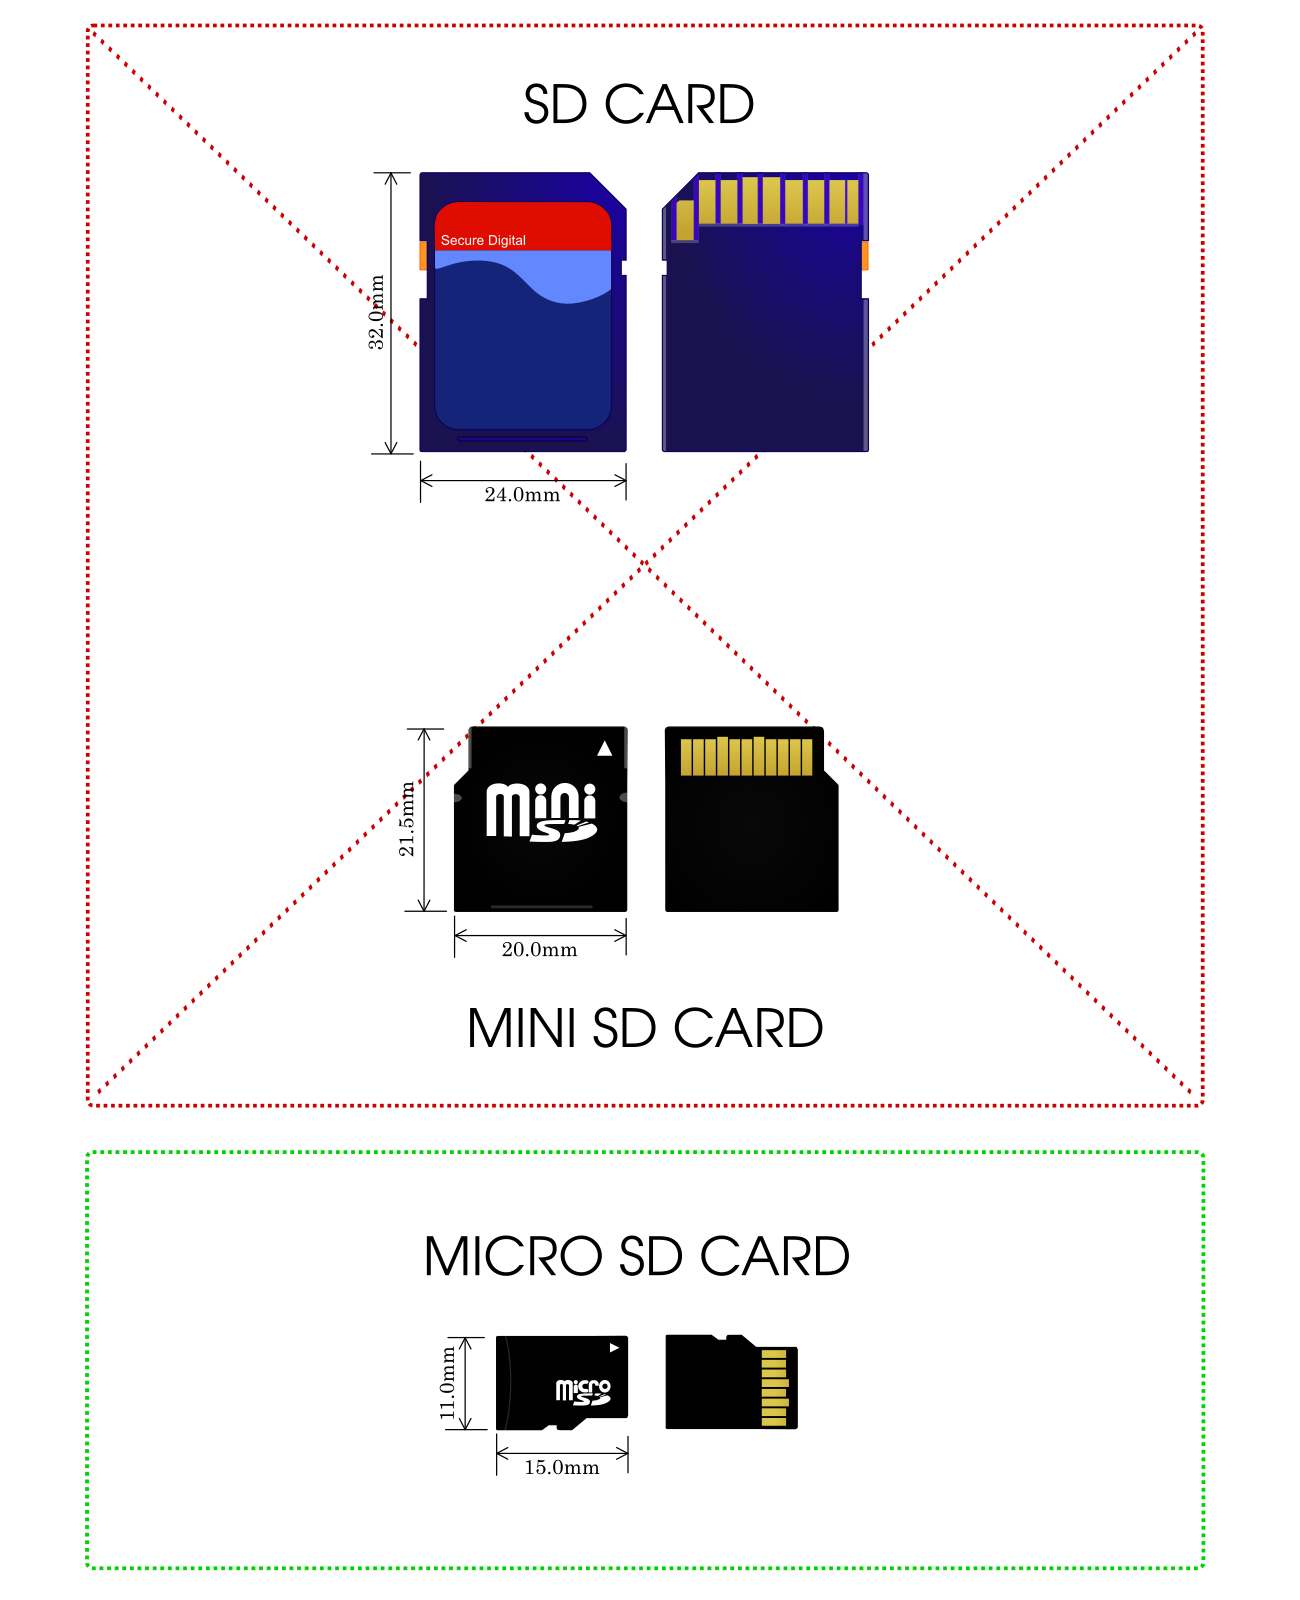
\includegraphics{images/sd_cards.png}
\caption{SD Cards}
\end{figure}

%%%%%%%%%%%%%%%%%%%%%%%%%%%%%%%%%%%%%%%%%%%%%%%%%%%%%%%%%%%%%%%%%%%%%%%%%%%%%%%%
% Removing the Micro SD Card - Replace SD Card - Formatting
%%%%%%%%%%%%%%%%%%%%%%%%%%%%%%%%%%%%%%%%%%%%%%%%%%%%%%%%%%%%%%%%%%%%%%%%%%%%%%%%
\subsection{Formatting}

It is recommended that the
\href{https://www.sdcard.org/downloads/formatter\_4/}{SD Memory Card Formatter}
application be used to format the card.  It is provided for free by the
\href{https://www.sdcard.org/index.html}{SD Association}.  The following will
assume use of this application.

\steps{Download \& Open}{%
\begin{enumerate}
  \item Download the \textit{SD Memory Card Formatter} application from
    \url{https://www.sdcard.org/downloads/formatter\_4/}.  It is available
    for both Windows and Mac so make sure you choose the appropriate download
    for your operating system.
  \item Insert the new \cMSD{f} into the computer.
  \item Open the \textit{SD Memory Card Formatter} application.
\end{enumerate}}

\begin{figure}[H]
\centering
  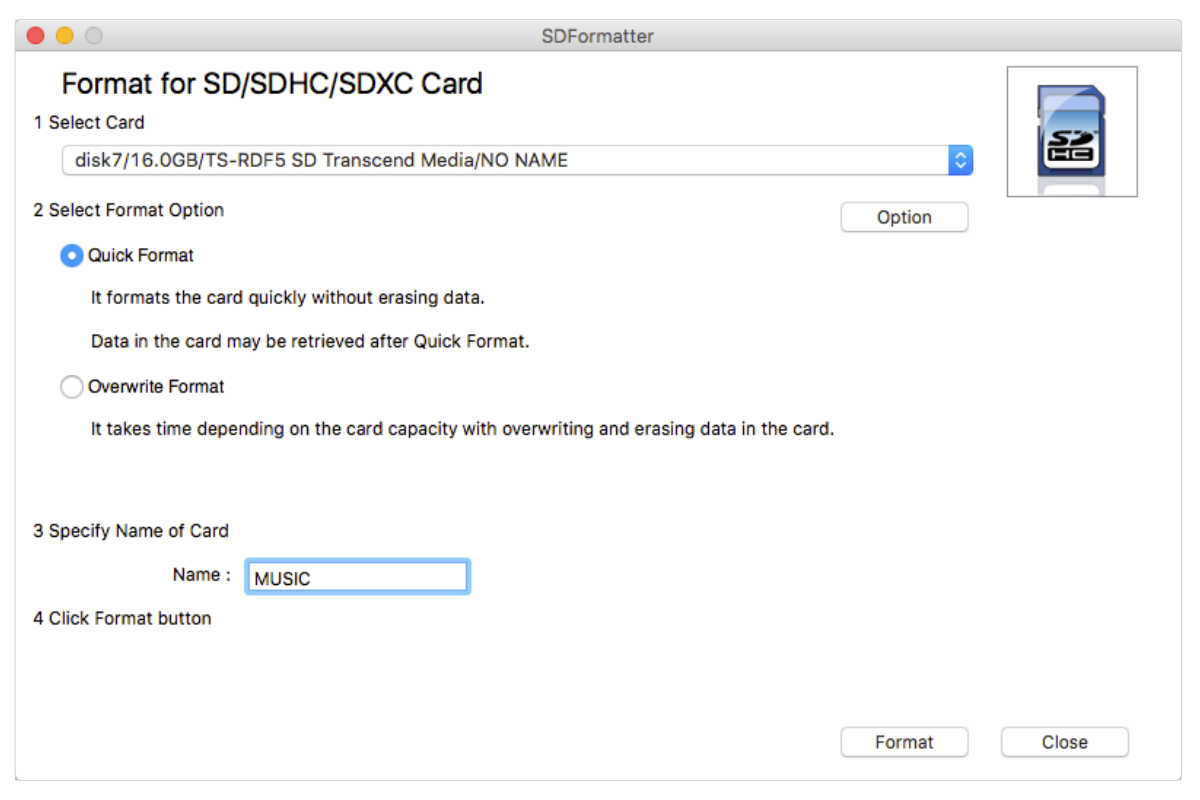
\includegraphics{images/sd_formatter.png}
\caption{Micro SD Card - SD Memory Card Formatter}
\end{figure}

The window is partitioned into \num{4} sections which will correspond to the
next steps.  Make sure when selecting the card in the first step, that you
select the card you just inserted.  If you select a different card, all of
its contents will be erased.

\danger{Selecting the wrong card will result in erasing the contents
of that card.}

\begin{figure}[H]
\centering
  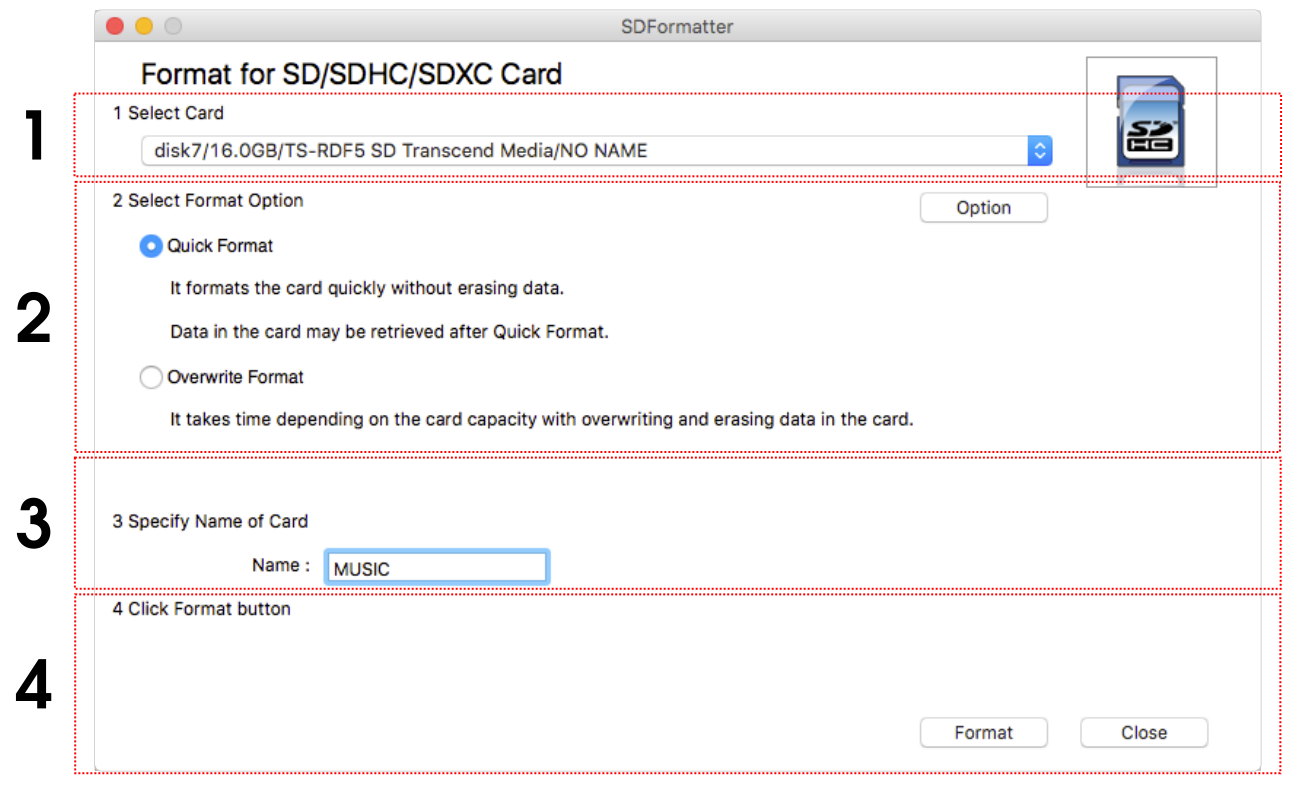
\includegraphics{images/sd_formatter_steps.png}
\caption{Micro SD Card - Formatting}
\end{figure}

\steps{Format}{%
\begin{enumerate}
  \item \textbf{Select Card} \newline
    Select the card you just inserted from the drop-down menu at the top.  If
    there is more than one choice, make sure you choose the correct card.
  \item \textbf{Select Format Option} \newline
    Leave this alone.
  \item \textbf{Specify Name of Card} \newline
    You can name this anything you like.
  \item \textbf{Click Format button} \newline
    Click on the "Format" button in the lower right.  It should not take long
    and when finished you should see some blue text underneath the option
    indicating success.
\end{enumerate}}

\begin{figure}[H]
\centering
  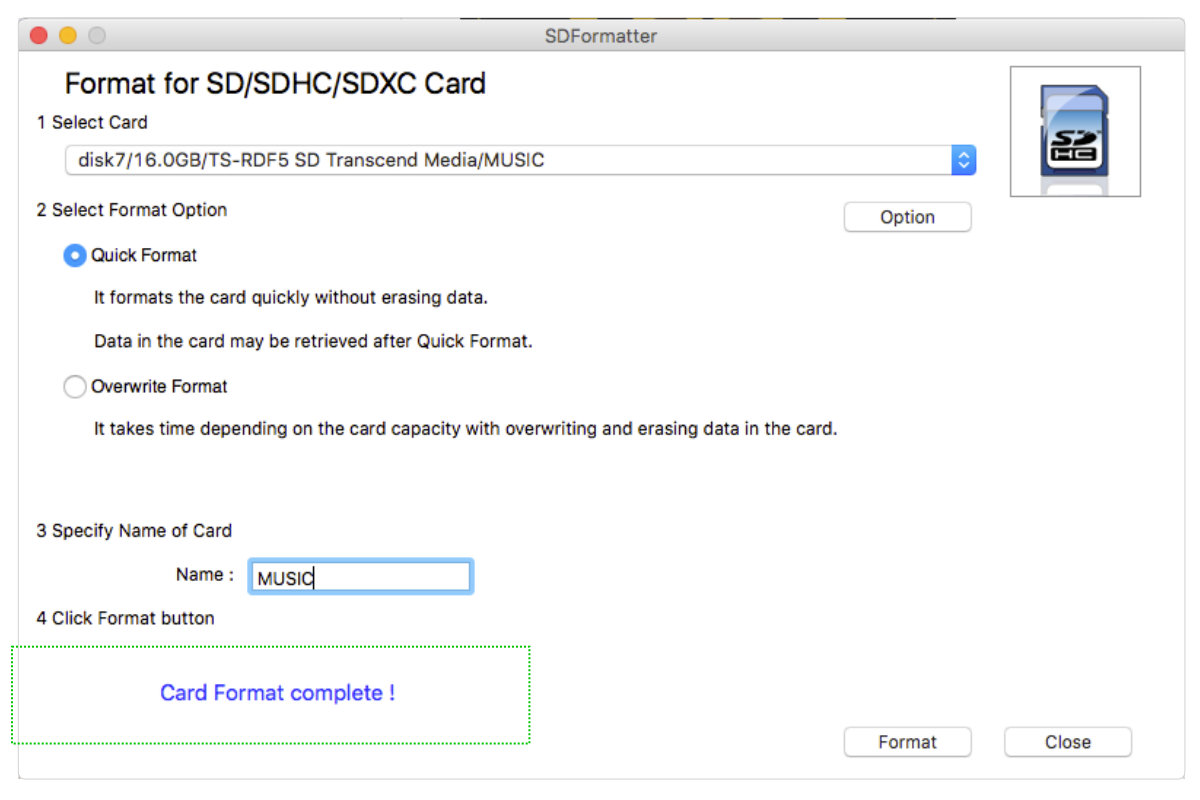
\includegraphics{images/sd_formatter_success.png}
\caption{Micro SD Card - Formatting Success}
\end{figure}

You can now add music to the card - see \hyperref[Adding Songs]{Adding Songs}.
